\chapter{Az alkalmazás felépítése}

Az alkalmazás három fő rétege az adatbázis, a backend és a frontend. Az alábbi fejezet ezen három réteg architektúrális
felépítésésről valamint az egyes rétegek összeköttetéséről foglalkozik.

\begin{figure}[!ht]
  \centering
  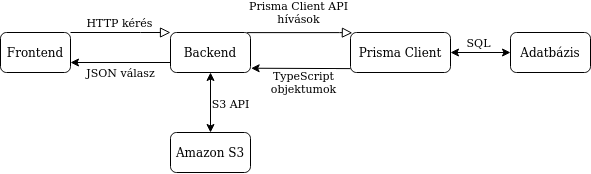
\includegraphics[width=150mm, keepaspectratio]{figures/architecture-diagram.png}
  \caption{Az alkalmazás high-level architektúrája}
  \label{fig:Architecture}
\end{figure}

\section{Adatbázisséma}

Az adatbázisséma tervezéséhez a dbdiagram.io nevű platformfüggetlen, webes ER diagram tervező szoftvert használtam.
Ez egy saját fejlesztésű, DBML nevű DSL nyelvet használ a séma leírására, és lehetővé teszi ennek exportálását különféle formátumokba.

\begin{figure}[!ht]
\centering
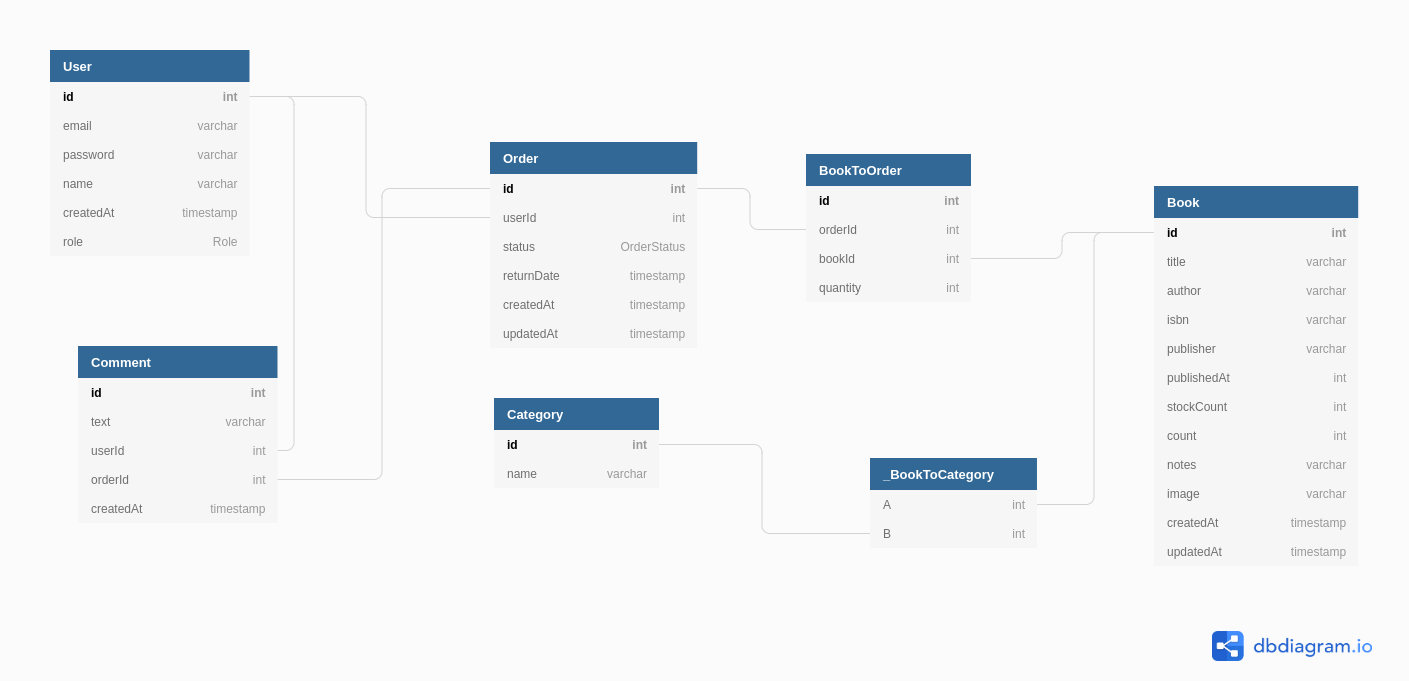
\includegraphics[width=150mm, keepaspectratio]{figures/dbschema.png}
\caption{Az adatbázisséma ER diagramja.}
\label{fig:DBSchema}
\end{figure}

A séma tervezése során a Prisma által használt elnevezési konvenciókat használtam megkönnyítve a két technológia közötti átjárhatóságot.


\section{A backend felépítése}

\subsection{Next.js API routes}

A Next.js keretrendszer a 9-es verzió óta lehetővé teszi szerveroldali kód írását az alkalmazásunkhoz.
Ennek segítségével a \lstinline|pages/api| mappába helyetett fájljaink szolgálnak backendként. Minden ide helyezett fájl
egyben a nevének megfelelő API végpont lesz, tehát például a \lstinline|pages/api/books.ts|-ben lévő kódot a pages/api/books URL-en keresztül tudjuk elérni.

Támogatja továbbá a backend-oldali dinamikus routing-ot, azaz például a \lstinline|pages/api/books/[id].tsx| fájl a \lstinline|pages/api/<id>| URL-nek felel meg, ahol
az \lstinline|id| változót alábbi módon érhetjük el:

\begin{lstlisting}[language=Java, caption=Next.js dinamikus routing]
export default function handler(req, res) {
  const {
    query: { id },
  } = req

  res.end(`Book: ${id}`)
}
\end{lstlisting}

\subsection{next-connect}
Alapesetben a Next.js csak egy egyszerű interface-t biztosít nekünk, amin keresztül elérhetjük a HTTP kérés request és response objektumokat annak kezeléséhez.
Ez azonban nezhézkessé teszi a különböző kérések feldolgozását (pl. GET, POST és PUT), valamint különbőző kódrészletek egyszerű újrafelhasználását.

Ennek kényelmesebbé tételére döntöttem a next-connect könyvtár használata mellett, amellyel a fenti igények könnyedén megvalósíthatóak.
Az alábbi két kódrészletben szeretném bemutatni a főbb különbségeket.

\begin{lstlisting}[language=Java, caption=Default Next.js API routes]
export default function handler(req: NextApiRequest, res: NextApiResponse) {
  if (req.method === 'GET') {
    res.statusCode = 200
    res.setHeader('Content-Type', 'application/json')
    res.end(JSON.stringify({ name: 'John Doe' }))
  } else if (req.method === 'POST') {
    // Process a POST request
  }
}
\end{lstlisting}

\begin{lstlisting}[language=Java, caption=Kérés kezelése next-connect segítségével]
import nextConnect from "next-connect"

const handler = nextConnect<NextApiRequest, NextApiResponse>()

handler
  .get((req, res) => {
    res.json({ name: 'John Doe' })
  })
  .post((req, res) => {
    // Process POST request
  })

export default handler
\end{lstlisting}

\subsubsection{Middleware támogatás}
A Next.js alapesetben nem rendelkezik beépített middleware támogatással, emiatt bizonyos kódrészletek újrahasználása körülményes lehet.
A next-connect azonban ezt a folyamatot rendkívül egyszerűvé teszi, így könnyen lehet védett útvonalakat létrehozni például csak bejelentkezett
felhasználók számára.

\begin{lstlisting}[language=Java, caption=Middleware kezelés next-connect segítségével]
import nextConnect from "next-connect"
import requireLogin from "middleware/requireLogin"
import requireAdmin from "middleware/requireAdmin"
const handler = nextConnect<NextApiRequest, NextApiResponse>()

handler
  .get((req, res) => {
    res.json({ name: 'John Doe' })
  })
  .use(requreLogin)
  .post((req, res) => {
    // Process POST request
  })
  .use(requireAdmin)
  // Process other requests

export default handler
\end{lstlisting}

A fenti kódrészletben a POST kérés csak bejelentkezett felhasználók számára elérhető. Ezek egymás után is fűzhetőek, így komplex
igények is rendkívül egyszerűen megvalósíthatóak.


\section{A frontend felépítése}

Az alábbi szekcióban szeretnék egy általános képet mutatni a frontend felépítéséről és az ott általában használt technológiákról illetve módszerekről.

\subsection{Routing}

A Next.js framework a frontenden is alkalmazza a file-based routing koncepcióját. Ennek megfelelően elegendő az \lstinline|src/pages/|
mappában elhelyezett \lstinline|.tsx| fájlban definiálnunk egy React komponenst, és a keretrendszer a megadott fájlnévnek megfelelő URL-en
fogja kirenderelni az oldalunkat.

Az adminoknak elérhető oldalakat egy külön \lstinline|admin| mappába helyeztem a könnyebb elkülöníthetőség érdekében.

Ezen felül a programkódból történő útvonalválasztásra is lehetőségünk van. Ez akkor hasznos, ha például bejelentkezés után szeretnénk
a felhasználónkat átirányítani egy másik oldalra.

Ezt a Next.js \lstinline|useRouter| hook-ja biztosítja számunkra. Segítségével tudunk a frontenden navigálni, illetve ezen keresztül
tudunk például URL paraméterekhez hozzáférni.

Az alábbi kódrészlet ezt a funkcionalitást demonstrálja.

\begin{lstlisting}[caption=Next.js kliensoldali router használata]
import { useRouter } from "next/router"

export default function SomePage() {
  const router = useRouter()
  const someId = router.query.id

  function handleLogin() {
    // other logic

    router.push("/")
  }
  return (
    {/* presentation logic */}
  )
}
\end{lstlisting}

A \lstinline|components/| mappába kerültek az újrafelhasznált, illetve kiszervezett React komponensek.
Az általam írt saját React hook-ok pedig az \lstinline|src/lib/hooks.tsx| fájlba kerültek.

\subsection{Link prefetch}

A Next.js segítségével egy, a felhasználói élményt nagy mértékben javító szolgáltatással leszünk gazdagabbak, ez pedig a link prefetch.

Ennek lényege, hogy ha egy adott, az oldalunkon belülre mutató link fölé visszük az egerünket, a böngésző az adott oldalhoz tartozó JavaScript
fájlokat még a linkre kattintás előtt lekéri a szervertől.
Ennek köszönhetően nagyméretű JavaScript-et tartalmazó oldalt is lehetséges relatíve gyorsan betölteni.

Ahhoz hogy ez a funkcionalitás elérhető legyen, minden, az oldalunkon belülre mutató linket egy külön komponensbe kell beágyaznunk.

\begin{lstlisting}[caption=NextLink használata Chakra UI linkkel együtt]
import NextLink from "next/link"
import { Link } from "@chakra-ui/react"

export default function Navbar() {
  // ...
  return (
    {/* ... */}
    <NextLink href="/profile">
      <Link>Profilom</Link>
    </NextLink>
    {/* ... */}
  )
}
\end{lstlisting}

Ahogy a lenti képernyőképen is látható, a profil oldalon az egeret ``Kölcsönzéseim'' link fölé irányítva megtörténik az \lstinline|orders|
oldalhoz tartozó JavaScript lekérése.

\begin{figure}[!ht]
  \centering
  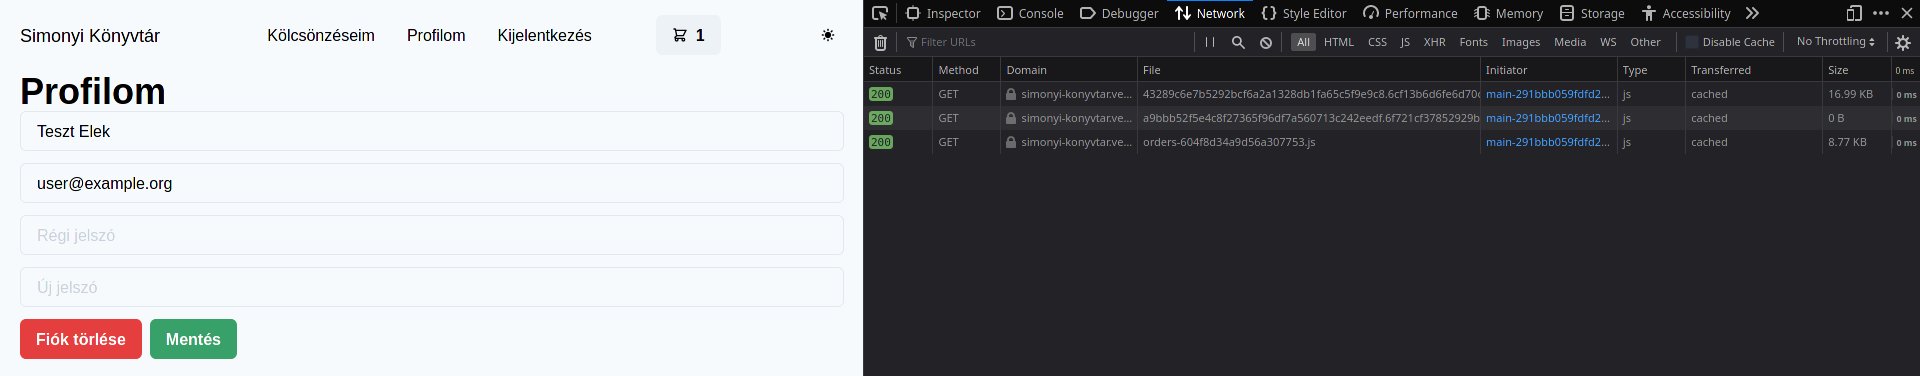
\includegraphics[width=150mm, keepaspectratio]{figures/next-link-cache.png}
  \caption{Next.js link prefetch}
  \label{fig:LinkPrefetch}
\end{figure}

\subsection{Optimistic UI update SWR-rel}

Egy másik, manapság gyakran alkalmazott módszer az úgynevezett Optimistic UI update.

Ennek lényege, hogy az oldalon megjelenített adat módosítása esetén előbb frissítjük a HTML tartalmat az új információval, minthogy a szervertől
pozitív választ kaptunk volna.

Nagy előnye a módszernek, hogy nem kell várni az esetlegesen sokáig tartó backend-oldali műveletekre, ami máskülönben ``befagyasztaná'' az alkalmazásunk
felületét. Fontos megjegyzés viszont, hogy navigációt nem érdemes így kezelni, mivel az esetleges hibákról nehéz értesíteni a felhasználót
és az esetleges inkonzisztens adatokkal nagyban csökkenthetjük a felhasználói élményt.

Az \lstinline|SWR| könyvtárat használva rendkívül egyszerűen valósíthatjuk meg ezt a funkcionalitást. A \lstinline|useSWR| hook által hozzáférésünk
van egy \lstinline|mutate| függvényhez, ami az általunk lekért erőforráshoz van kötve.

Ennek segítségével bármikor tudjuk módosítani a képernyőn megjelent adatainkat.
Ezt az SWR ezután validálja a POST kérésünk által visszaadott eredménnyel, és ha egyezik,
a belső állapotot is megváltoztatja, ha pedig eltérést tapasztal, akkor a korábbi állapotot őrzi meg és jeleníti meg a képernyőn.

\begin{lstlisting}[caption=Optimistic UI update megvalósítása]
export default function CategoriesIndexPage() {
  const hasAccess = useRequireRoles([userrole.ADMIN])
  if (!hasAccess) {
    return <ErrorPage statusCode={401} message="Nincs megfelelő jogosultságod!" />
  }
  const [newCategory, setNewCategory] = useState("")
  const { data, error, mutate } = useSWR<Category[]>("/api/categories", fetcher)

  const toast = useToast()

  if (error) return <Text fontSize="lg">Nem sikerült betölteni a kategóriákat</Text>
  if (!data) return <Loading />

  async function handleDelete(cat: Category) {
    // handle deleting a category
  }

  async function handleAddCategory(event: FormEvent) {
    event.preventDefault()
    const category: CategoryCreateInput = { name: newCategory }
    const res = await fetch("/api/categories", {
      method: "POST",
      body: JSON.stringify(category),
      headers: {
        "Content-Type": "application/json",
      },
    })
    if (res.ok) {
      setNewCategory("")

      mutate(async (categories) => {
        const newCategory = await res.json()

        return [newCategory, ...categories.slice(1)]
      })
    }
  }

  async function handleEditCategory({ id, name }) {
    // handle editing a category
  }

  return (
    <>
      <form onSubmit={handleAddCategory}>
        <Flex direction="row" mb={6}>
          <FormControl mr={4} flex="1">
            <Input
              isRequired
              placeholder="Új kategória"
              value={newCategory}
              onChange={(e: FormEvent<HTMLInputElement>) =>
                setNewCategory(e.currentTarget.value)
              }
            />
          </FormControl>
          <Button type="submit">Hozzáadás</Button>
        </Flex>
      </form>
      <Heading as="h1">Kategóriák</Heading>
      {data && (
        <CategoryList
          data={data}
          handleDelete={handleDelete}
          handleEdit={handleEditCategory}
        />
      )}
    </>
  )
}

\end{lstlisting}

\subsection{Page layout megvalósítása}

Az alkalmazásban a felső navigációs sávot és az alsó footer-t szerettem volna minden oldalon megjeleníteni.

Ehhez az egyik lehetőség, hogy minden aloldalba beillesztem ezt a két komponenst, azonban ez sok kódduplikációhoz és esetenként
inkonzisztens megjelnéshez vezetne.

Szerencsére a Next.js-ben lehetőségünk van egy központi layout kialakítására, ami azután minden oldalunk használni fog. Ehhez nem kell
mást tennünk, mint az \lstinline|src/pages| mappában létrehozni egy \lstinline|_app.tsx| nevű fájlt és itt implementálni az általunk
kívánt layout-ot.

\begin{lstlisting}[caption=Minden oldalra kiterjedő layout alkalmazása Next.js keretrendszerben]
import { Box, ChakraProvider } from "@chakra-ui/react"
import { AppProps } from "next/app"
import dynamic from "next/dynamic"
import Head from "next/head"

import { Container } from "components/Container"
import Footer from "components/Footer"

const Navbar = dynamic(() => import("components/Navbar"), { ssr: false })

const App = ({ Component }: AppProps) => {
  return (
    <>
      <Head>
        <title>Simonyi Könyvtár</title>
        <meta property="og:title" content="Simonyi Könvtár" key="title" />
        <meta lang="hu" />
      </Head>
      <ChakraProvider>
        <Container>
          <Navbar />
          <Box flex="1" width="100%" px={5} maxW="6xl">
            <Component />
          </Box>
          <Footer />
        </Container>
      </ChakraProvider>
    </>
  )
}

export default App
\end{lstlisting}

A fenti kódrészletben az \lstinline|App| komponens bemeneti paramétereiben lévő \lstinline|Component| reprezentálja az oldalanként
dinamikusan változó tartalmat. Az itt szereplő \lstinline|Container| komponens egy \lstinline|flexbox| konténer, aminek segítségével
a footer akkor is az oldal aljához tapad, ha a felette lévő tartalom nem tölti ki teljesen a képernyőt.


\section{Kódmegosztás}


\section{Képfeltöltés}

A könyvekhez lehetősév van borítóképet feltölteni, ezeket azonban valahol tárolni is kell.

Ennek a tárolására az Amazon S3 szolgáltatását választottam. A csatolt képet a frontend először elküldi a backendnek,
majd az az \lstinline|aws-sdk| könyvtárat használva feltölti a képet az S3 bucket-be, az adatbázisba csak a képet
azonosító generált kerül be. Így lehetőségünk van a képek egyszerű és adatbázisfüggetlen kezelésére.

\begin{figure}[!ht]
  \centering
  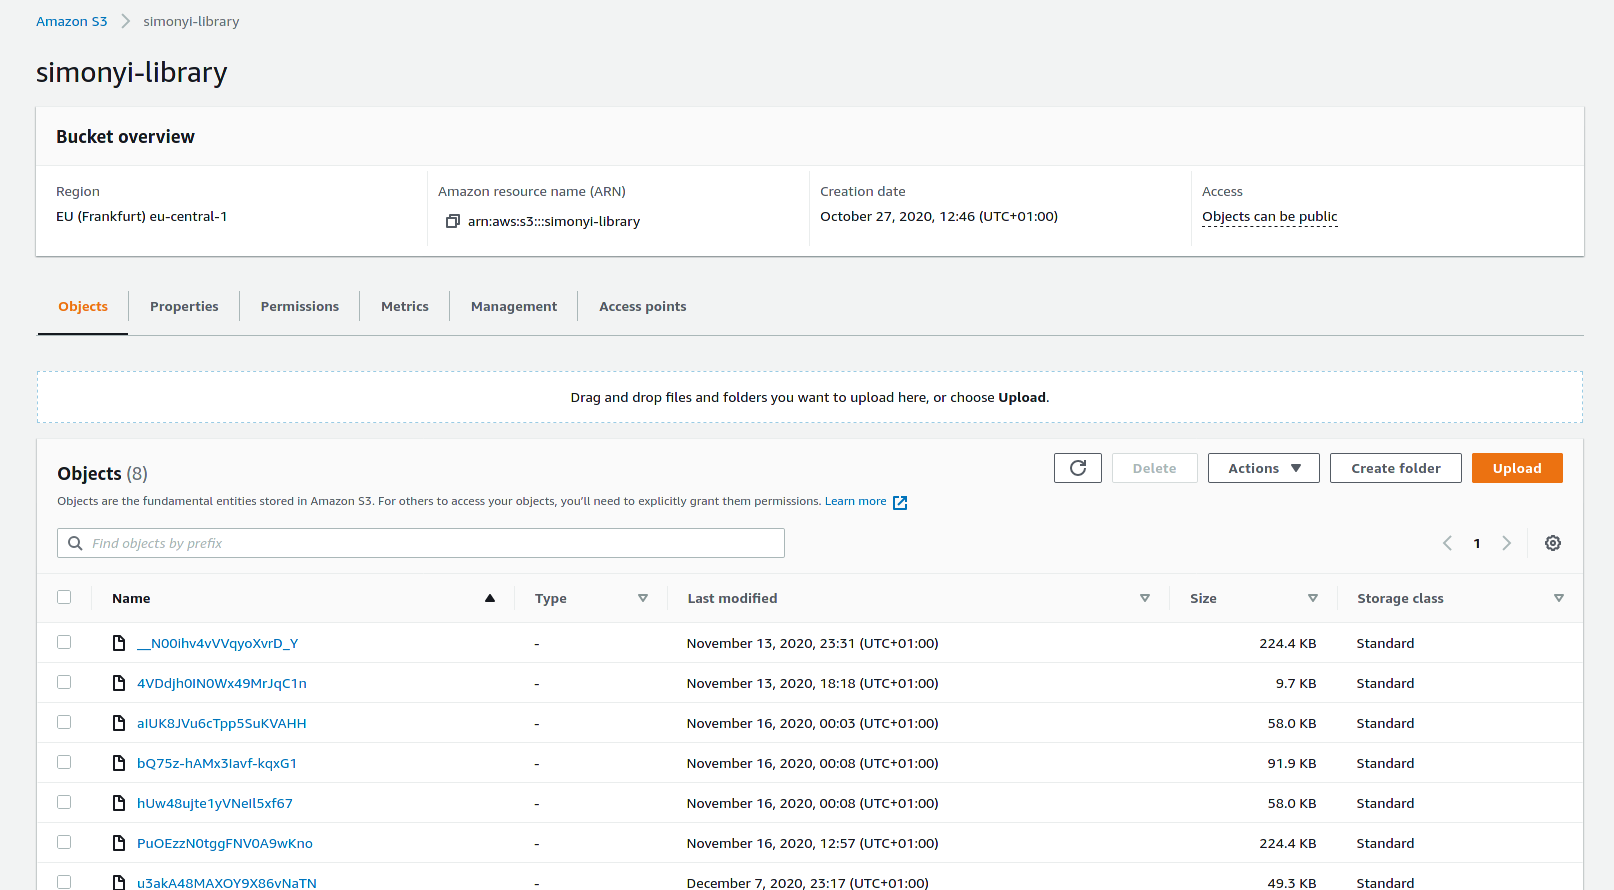
\includegraphics[width=125mm, keepaspectratio]{figures/s3-dashboard.png}
  \caption{Amazon S3 konzol}
  \label{fig:S3Console}
\end{figure}
